\chapter{Introduction}
Virtual environments as narrative spaces, represents a novel way to tell a story or convey a specific feeling to the audience. Unlike traditional storytelling methods that rely on delivering a story through dialogue, cutscenes or text dumps; environmental storytelling operates more subtly.\par

To effectively highlight environmental storytelling, it’s crucial to weave narrative elements seamlessly into the virtual environment that evoke emotions and encourage players to question their surroundings. The very design of virtual spaces like their size, shape, flow, connectivity and materials can convey narrative meaning. The layout of virtual environment can guide the player along a specific path, revealing information sequentially or create feelings of safety, exposure or confusion. The environment becomes a silent narrator, communicating with audience through carefully crafted, immovable details that enhance immersion and improve the narrative experience\cite{Environmental_Storytelling_Blogpost}.\par

Due to interactive, exploratory and emergent capabilities of video games in storytelling, environmental storytelling practiced more often especially after video game industry's increased popularity\cite{Video_Game_Industry_Stat}. While this practice is increasing, the auditory domain of environmental storytelling remains understudied. This thesis focuses specifically on the auditory dimension of environmental storytelling practice.\par

Movies, video games and interactive art installations often utilize different human sensory fields simultaneously. Understanding and leveraging this multi-modality is crucial when contributing to these mediums as an artistic individual or researcher.\par

With this multi-sensory understanding, this research will further investigate the interplay/crossplay between auditory and tactile feedback within environmental storytelling. The aim is to explore how audio-tactile experiences can enhance immersion, evoke emotional responses and create richer, more embodied narrative contents for the audience.\par
    \section{Research Question} 
    The study addresses the following three fundamental questions about auditory environmental storytelling:
    \begin{enumerate}
        \item To what extent does multi-modality play a role in the environmental storytelling?
        \item How multi-modal stimulation can be utilized to enhance auditory environmental storytelling?
        \item How effectively can an interactive audio-tactile system convey distinct environmental characteristics (space size, material properties etc.) and narrative cues to an audience?
    \end{enumerate}
    To begin this investigation, the following section reviews foundational concepts of multi-modal interaction, leading into a broader review of existing literature.
    \section{Multi-Modality} 
    Modalities, the plural of modal, is a term primarily related to how media is presented, its form, or its mode. Basically, modalities are modes, a manner, way or method of doing something. Multi-modality refers to the interplay between different modes\cite{Multimodal_Discourse}.\par 

    The term "modality" is studied across diverse disciplines such as linguistics, media studies, semiotics and cognitive science. Each examining different aspects of representation, communication, or interaction. In the context of human-computer interaction(HCI) this thesis uses modality term as specifically referring to sensory channels or the distinct forms of stimuli like auditory and tactile feedback.\par

    Through this focus modality can be broadly understood as a distinct sensor, channel, system or manner through which information is represented, perceived, processed or exchanged.\par

    The strategic combination of multiple modalities is often driven by the goal of creating more effective, intuitive, and engaging user experiences. Presenting information through various sensory channels can meet different user needs and contexts, creating expressions that can potentially improve narrative and engagement by offering complementary or redundant information.\par

    In the digitized world, different sensory modes have technically become the same at some level of representation, and they can be operated by one multi-skilled person, using one interface, one mode of physical manipulation, so that he or she can ask, at every point: "Shall I express this with sound or music?", "Shall I say this visually or verbally?"\cite{Multimodal_Discourse}.\par

    Sensory modalities such as auditory cues can effectively convey ambient information, direct attention and shape emotional tone, while the somatosensory system(the system responsible for our conscious awareness of touch, pressure, pain, temperature and body position\cite{Somatic_Sensory}.) offers a direct physical link to digital environments, enhancing feelings of presence and embodiment.\par

    Investigating how these multi-modal experiences can enhance immersion, evoke emotional responses, create richer and more embodied narrative contents, we aim to explore auditory and somatosensory capabilities when an environmental narration introduced to an audience.\par
    \section{Environment as a Tool for Narration} 
    \emph{"The audience is not a passive observer, but actively investigates the frame both spatially and temporally, responding to the tension created within the narrative space\cite{Transmedia_Storytelling}."}

    Given text from Interactive Narrative and Transmedia Storytelling highlights the new role and importance of the audience. Virtual spaces in interactive narratives are more than just digital settings. They are the environments where the story unfolds and where the audience actively participates. Environmental storytelling promotes virtual environments role from basic background to an active narrative agent.\par

    Strategically placed objects in the environment can tell a story on their own. A knocked-over chair, a specific book left open or a series of photographs can hint at past events, reveal aspects of a character's personality or provide clues that help the audience piece together the narrative\cite{Environmental_Storytelling_Blogpost}.\par 

    In a professionally structured narrative there are macro and micro storytelling scopes. When it has done well, this hierarchy creates a depth of narrative design that neither approach could achieve alone, allowing audience to connect grand macro and micro level events in ways that feel organic and profound\cite{Environmental_Storytelling_Blogpost}. Environmental storytelling has capability to convey stories that aren’t always directly told through dialogue or cutscenes.\par

    Following example images from video games, movies and even from our real life, given to deepen understanding of environmental storytelling as a tool for narration;

    \begin{figure}[H]
    \centering
    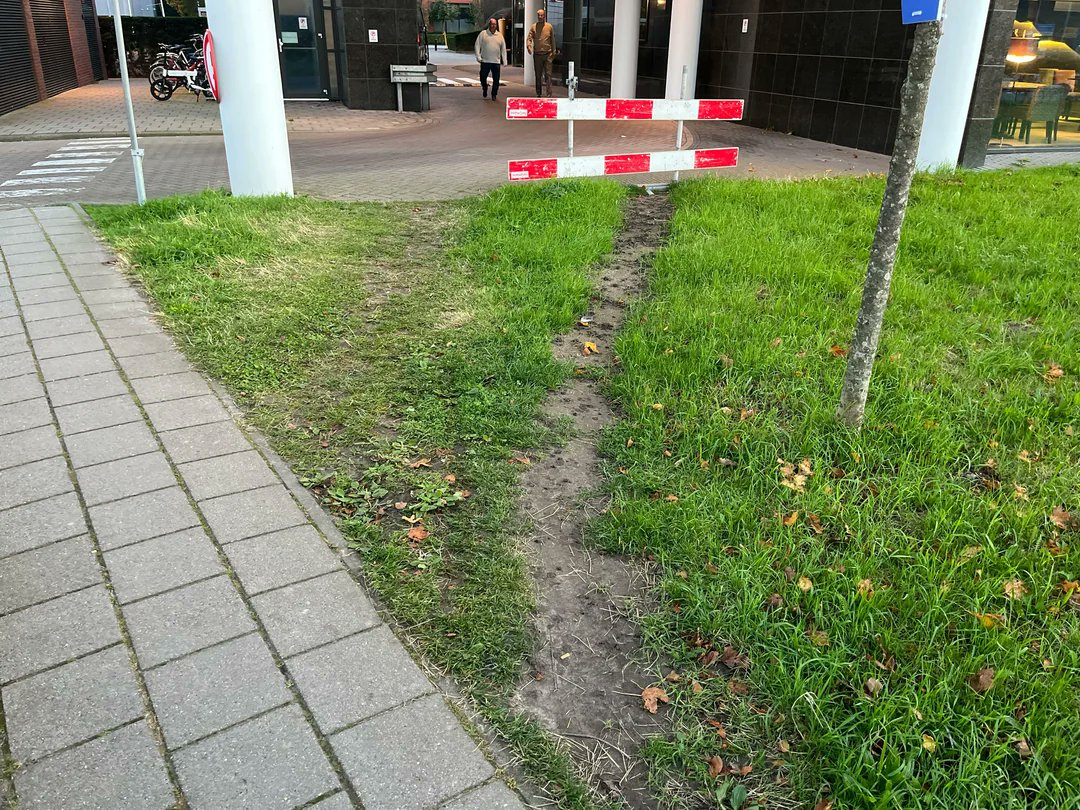
\includegraphics[width=0.8\textwidth]{images/environmental_storytelling_02}
    \caption{An image from a public road.}
    \label{fig:ES_01}
    \end{figure}

    On macro level scope, \ref{fig:ES_01} shows a shortcut made by people walking through the grass instead of using the sidewalk. The red-and-white barrier at the end of the path indicates an attempt to enforce the intended route, but the worn trail on the left shows people kept choosing the faster way.\par

    \begin{figure}[H]
    \centering
    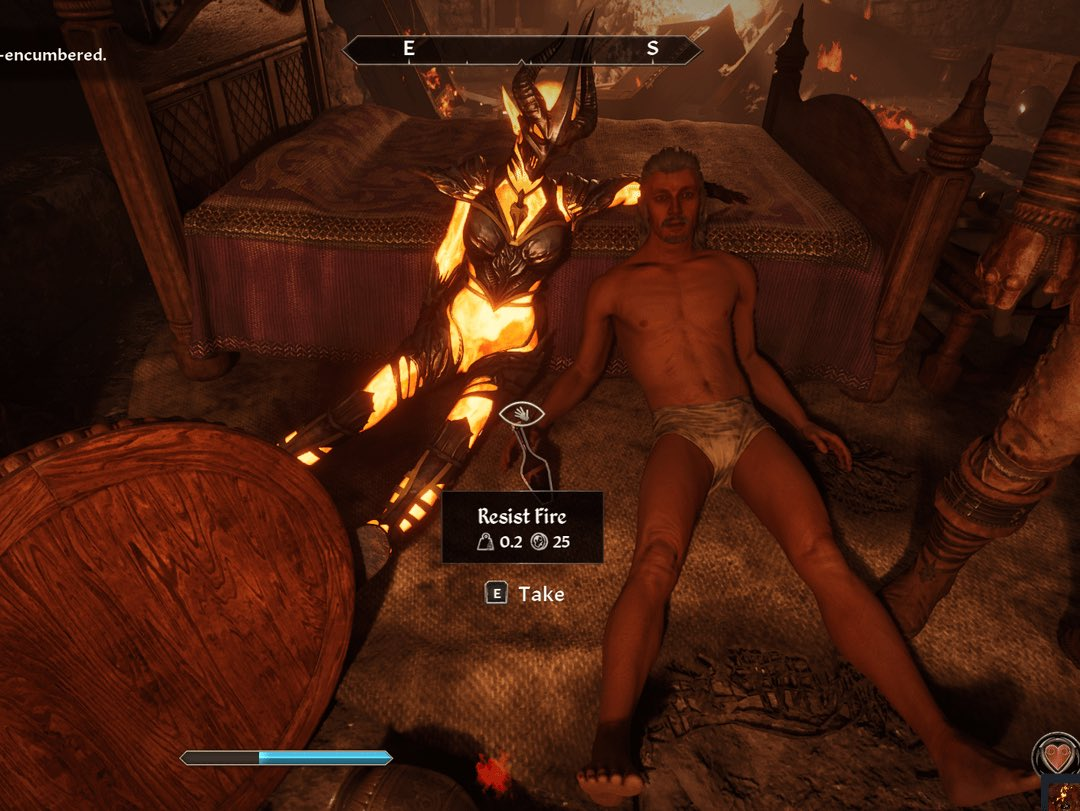
\includegraphics[width=0.8\textwidth]{images/environmental_storytelling_04}
    \caption{A visual from a video game called Oblivion.}
    \label{fig:ES_02}
    \end{figure}

    On micro level scope, \ref{fig:ES_02} tells a humorous story. A man lies exhausted beside a fiery figure on the floor next to a bed with a "Resist Fire" potion highlighted, hinting maybe he needed magical help to survive an intense, possibly romantic encounter.\par

    \begin{figure}[H]
    \centering
    \includegraphics[width=0.8\textwidth]{images/environmental_storytelling_05}
    \caption{An image of a building in Istanbul, Turkey.}
    \label{fig:ES_03}
    \end{figure}

    With another macro level scope example, \ref{fig:ES_03} shows a building from Istanbul, made up of layers from different time periods, each added on top of the previous one. The labels on the right indicates the specific architectural style(starting with the Roman Empire at the bottom and ending with the Republic Era at the top) telling a visual story of Istanbul’s long and complex history. It reflects the city’s rich heritage, shaped by centuries of conflict, change and development, all embodied in a single structure.\par

    \begin{figure}[H]
    \centering
    \includegraphics[width=0.8\textwidth]{images/environmental_storytelling_06}
    \caption{A visual from a video game called Control.}
    \label{fig:ES_04}
    \end{figure}

    With another micro level scope example, \ref{fig:ES_04} shows a character stands before a mail room door. The blood spreading under the door serves as an effective environmental narrative device, wordlessly hinting to the player the danger. Signalling that something violent has happened in the space they're about to enter, creating tension and anticipation without explicit exposition.\par    

    These examples provided to illustrate how this technique functions across various media and even in our physical world. What makes environmental storytelling special is that it lets each audience member piece together the story in their own way, creating a more personal connection.\par

    With the given level of understanding in environmental storytelling, next section covers my own ideas and proposed installation, a multi-modal playback system directly targeted for environmental storytelling.\par
    \section{Embracing Sphere and My Own Perception} 
    If I may be a bit more sincere and break the formal language of last couple subchapters, I would like to start by introducing myself.\par 
    
    My name is Mehmet, an audio designer and interactive media artist, born in Bursa, Turkey and currently based in Linz, Austria. My design approach is to create soundscapes and interactive audio experiences with gamification and developing interactions for auditory exploration.\par

    Since I was a child I have been amused by video games and stories that have been told through video games. I studied music technologies in my bachelor's degree, developed my skills around interactive audio and now with the Interface Cultures master's programme, next chapter of my life is going deeper in the field of conjunction of human and technology in the art domain which is highly related to interaction, interaction design and media studies.

    \begin{figure}[H]
    \centering
    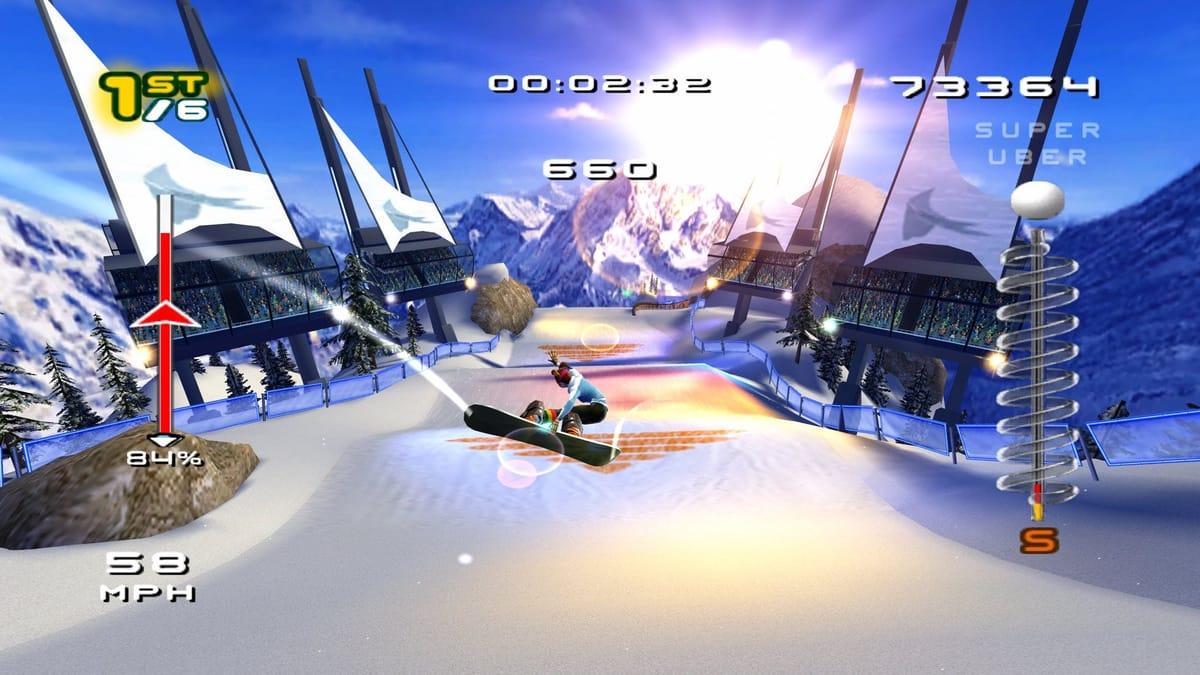
\includegraphics[width=0.8\textwidth]{images/ssx3}
    \caption{Video game SSX 3, PlayStation 2 (2003).}
    \label{fig:SSX3}
    \end{figure}

    I remember the first time when I played a game called "SSX 3" which is a snowboarding game. I can still clearly recall the feeling when jumping off a cliff onto the snow surface and simultaneous rumble coming from Dualshock 2(\ref{fig:DS2}). Feeling of the gritty snow texture when turning a tight corner or imminent hit response when I crashed into a barrier, as a child who experiencing this kind of multi-modal experience for the first time, it was really remarkable.\par

    That memory of the Dualshock 2 rumbling in sync with the snowboarding action in SSX 3 really stuck with me. It wasn't just about seeing the snow or hearing the sounds; it was feeling the impact and the texture of that virtual world.

    \begin{figure}[H]
    \centering
    \includegraphics[width=0.8\textwidth]{images/gamepad}
    \caption{Playstation 2 gamepad, Dualshock 2.}
    \label{fig:DS2}
    \end{figure}

    Dualshock 2 is the name of main gamepad of the PlayStation 2, which released in 2000 and stayed relevant until nearly 2012-2013. As the physical user interface of this hugely popular and successful console, the Dualshock 2 was also a well engineered interface for gaming.\par

    The vibration motors in the DualShock 2 were quite simple, basically small weights spinning off-center to create a general rumble. It was more of a strong shake or a light buzz\cite{PlayStation_Blogpost}. Today, vibrotactile devices/tools are much more advanced, capable of producing a wider range of precise textures and feelings. Modern game controllers, like the Nintendo Switch's "HD Rumble" or the PlayStation 5's DualSense, take advantage of this. They can create much clearer and more varied tactile effects, like the subtle click of a dial, the tension of a bowstring, or the feeling of raindrops, making virtual interactions feel surprisingly realistic and nuanced.

    \begin{figure}[H]
    \centering
    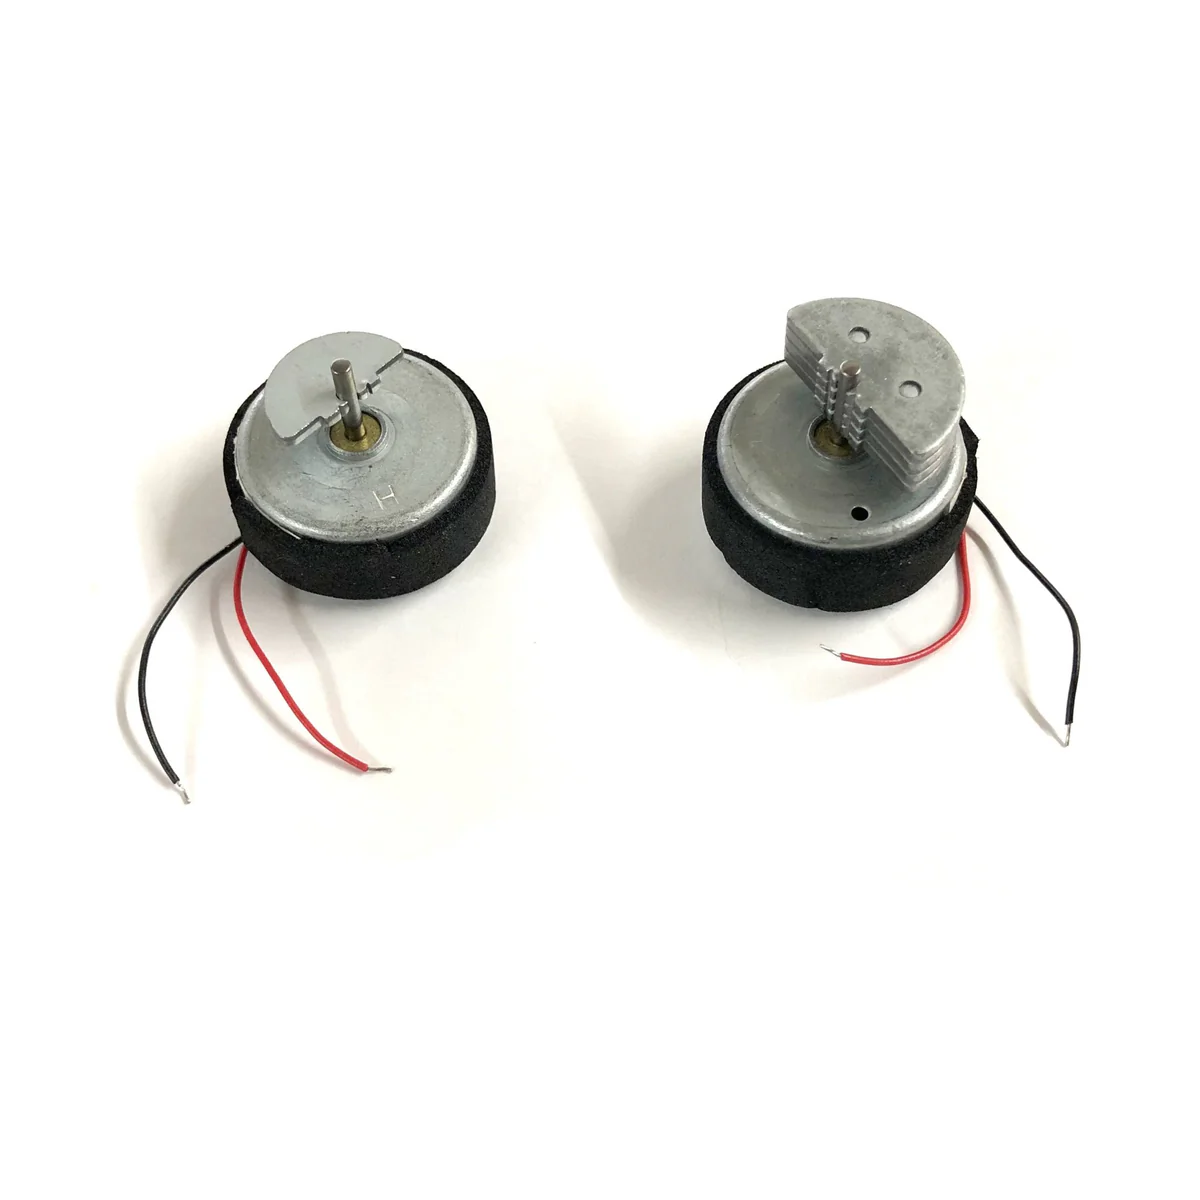
\includegraphics[width=0.7\textwidth]{images/vibration_motors_ds2}
    \caption{Vibration motors of Dualshock 2.}
    \label{fig:Vib_Motors}
    \end{figure}

    My first hand experience and understanding that combining sound with touch could make a virtual experience feel incredibly real and immersive. With years of other experiences and knowledge about interaction and multi-modal stimuli, made me wonder how much more could be done if these sensory connections were designed intentionally to tell a story or convey specific feelings about an environment.\par

    Embracing Sphere came to life as an idea with the background that I have stated. "Embracing Sphere", as a main title that on the one side, poetic yet on the other side a direct analogy of user interaction for a playback system that will be briefly explained later.\par
    
    The "playback system" aspect of Embracing Sphere is about creating a personal physical sphere where users can explore these combined audio-tactile sensations. It's about giving the audience a more embodied way to connect with a narrative, where what they hear is enhanced and expanded by what they can physically sense.\par
    
    My artwork, therefore, aims to be a practical exploration of the ideas in this thesis. "Embracing Sphere" is designed to be a tool to investigate how these audio-tactile experiences can shape our perception of a virtual space, its materials, and the subtle narrative cues embedded within it. It’s my way of testing how powerful this multi-modality of hearing and touch can be in making environmental storytelling more engaging for an audience.\par

    \section{Scope and Limitations}
    Haptic feedback refers to feedback perceived through the sense of touch. The haptic system uses sensory information derived from mechanoreceptors and thermoreceptors embedded in the skin together with mechanoreceptors embedded in muscles, tendons and joints\cite{Haptic_Perception-A_Tutorial}.\par 

    This research narrows its focus to vibrotactile feedback generated specifically by Voice Coil Actuators (VCAs). Consequently, other forms of haptic interaction, such as force feedback, thermal feedback, or electrovibration, are outside the scope of this study. VCAs are particularly suitable for vibrotactile applications due to their operational principles, which are similar to those of loudspeakers and voice coil actuators\cite{Audio-Tactile_Rendering}, allowing for conventional audio recording practices viable on haptic feedback content creation. A further exploration can be found in subchapter 2.4 Haptics and Perception, where vibrotactile hardwares and human perception capabilities are discussed in detail.\par 

    The study is limited by the specific operational range (e.g., frequency, amplitude) of the VCAs employed. Different VCAs possess varying performance characteristics and the chosen model may not represent the full spectrum of possible vibrotactile sensations.\par

    Another limitation is individual differences in vibrotactile sensitivity and perception thresholds among participants. While subchapter 2.4 will explore general human perception, this study does not control for all individual variabilities(age, skin condition, prior haptic experiences etc.).\par
    \section{Thesis Outline}
    With the last paragraphs of Chapter 1 - Introduction, this chapter aims to give an overall look for the thesis structure, topics that will covered and brief summary of the rest of chapters.\par

    Chapter 1 - Introduction, established the research context, presented the central research questions, inspirations and personal insights driving to this work. Later defined the scope and limitations of the investigation and provided this outline of the thesis structure.\par

    Chapter 2 - Background and Related Works, will offer a comprehensive review of existing literature and foundational concepts crucial to this research. This includes defining environmental storytelling and exploring its existing methods across various mediums, before focusing on auditory environmental storytelling. It will then investigate the principles of room acoustics, explaining Room Impulse Responses (RIRs), their measurement, the mathematical concept of convolution and its application in digital audio and sound art. Furthermore, it will provide a detailed review of haptics, different feedback modalities, fundamental aspects of human tactile perception and examples of haptic usage in diverse fields. Finally, the chapter will explore audio-tactile interaction, defining the concept and examining its application in contemporary media.\par

    Chapter 3 - System Design and Methodology, will detail the conceptual framework and systemic design of the proposed interactive system. It will cover the methodology for procedural Room Impulse Response (RIR) generation, the design of the audio and haptic playback systems, the interaction design principles and the intended narrative structure built by the system.\par

    Chapter 4 - Implementation, will describe the practical realization of the system. This chapter will cover the specific hardware setup, the software development process and tools utilized, the materialization of the research into an interactive art project and will discuss key challenges encountered during implementation and their solutions.\par

    Chapter 5 - Conclusion, will summarize the entire research endeavor. It will directly address the research questions, acknowledge the limitations of the study.\par